\vspace{10pt}
\section{Design Methodology}\label{sec:framwork}
Based on the analysis of Section~\ref{sec:w_and_r}, a new design flow is proposed to explore the design space of cross-point ReRAM arrays, as shown in Figure~\ref{fig:FlowChart}. Generally, the flow can be summarized as two stages: initialization stage and computation stage. At the initialization stage, the physical parameters, including the resistances of ReRAM cell, interconnect wires, and pull up resistors, the threshold voltage of the ReRAM cell, as well as non-linearity coefficients, are initialized. Since these values are constant for a given process technology, they need not be changed during the design space exploration. As a next step, the design constraints are specified based on area/energy budgets and different applications. Then the  original version of coefficients matrix $A_{basic}$ and the vector of constant terms $C_{basic}$ are set up. Since the value of $A_{basic}$ and $C_{basic}$ do not consider the edge conditions of the write/read schemes and their values do not change during the design space exploration. Then the programming schemes are chosen. The designer can either explore all possible programming schemes or choose a specific scheme based on previous results (for example, we have already shown that one bit write operation is more suitable for an area-constrained design than multi bit write). Then the final step of the initialization stage is to adjust the coefficients in $A_{basic}$ and $C_{basic}$ based on the edge conditions. At the beginning of the computing stage, the reliable array size is obtained by examining the worst case voltage drop and the read margin requirement. Then an iteration is performed to calculate the energy consumption and area overheads for each array size. The result are analyzed for all the array organizations. If there is any array organization that meets the design constraints provided at  the initialization stage, then the allowable array sizes with their energy consumption and area overheads are summarized as the design space for the given constraints. Otherwise, the programming schemes need to be adjusted for a new round of evaluation.



\begin{figure}[!t]
\centering
  % Requires \usepackage{graphicx}
  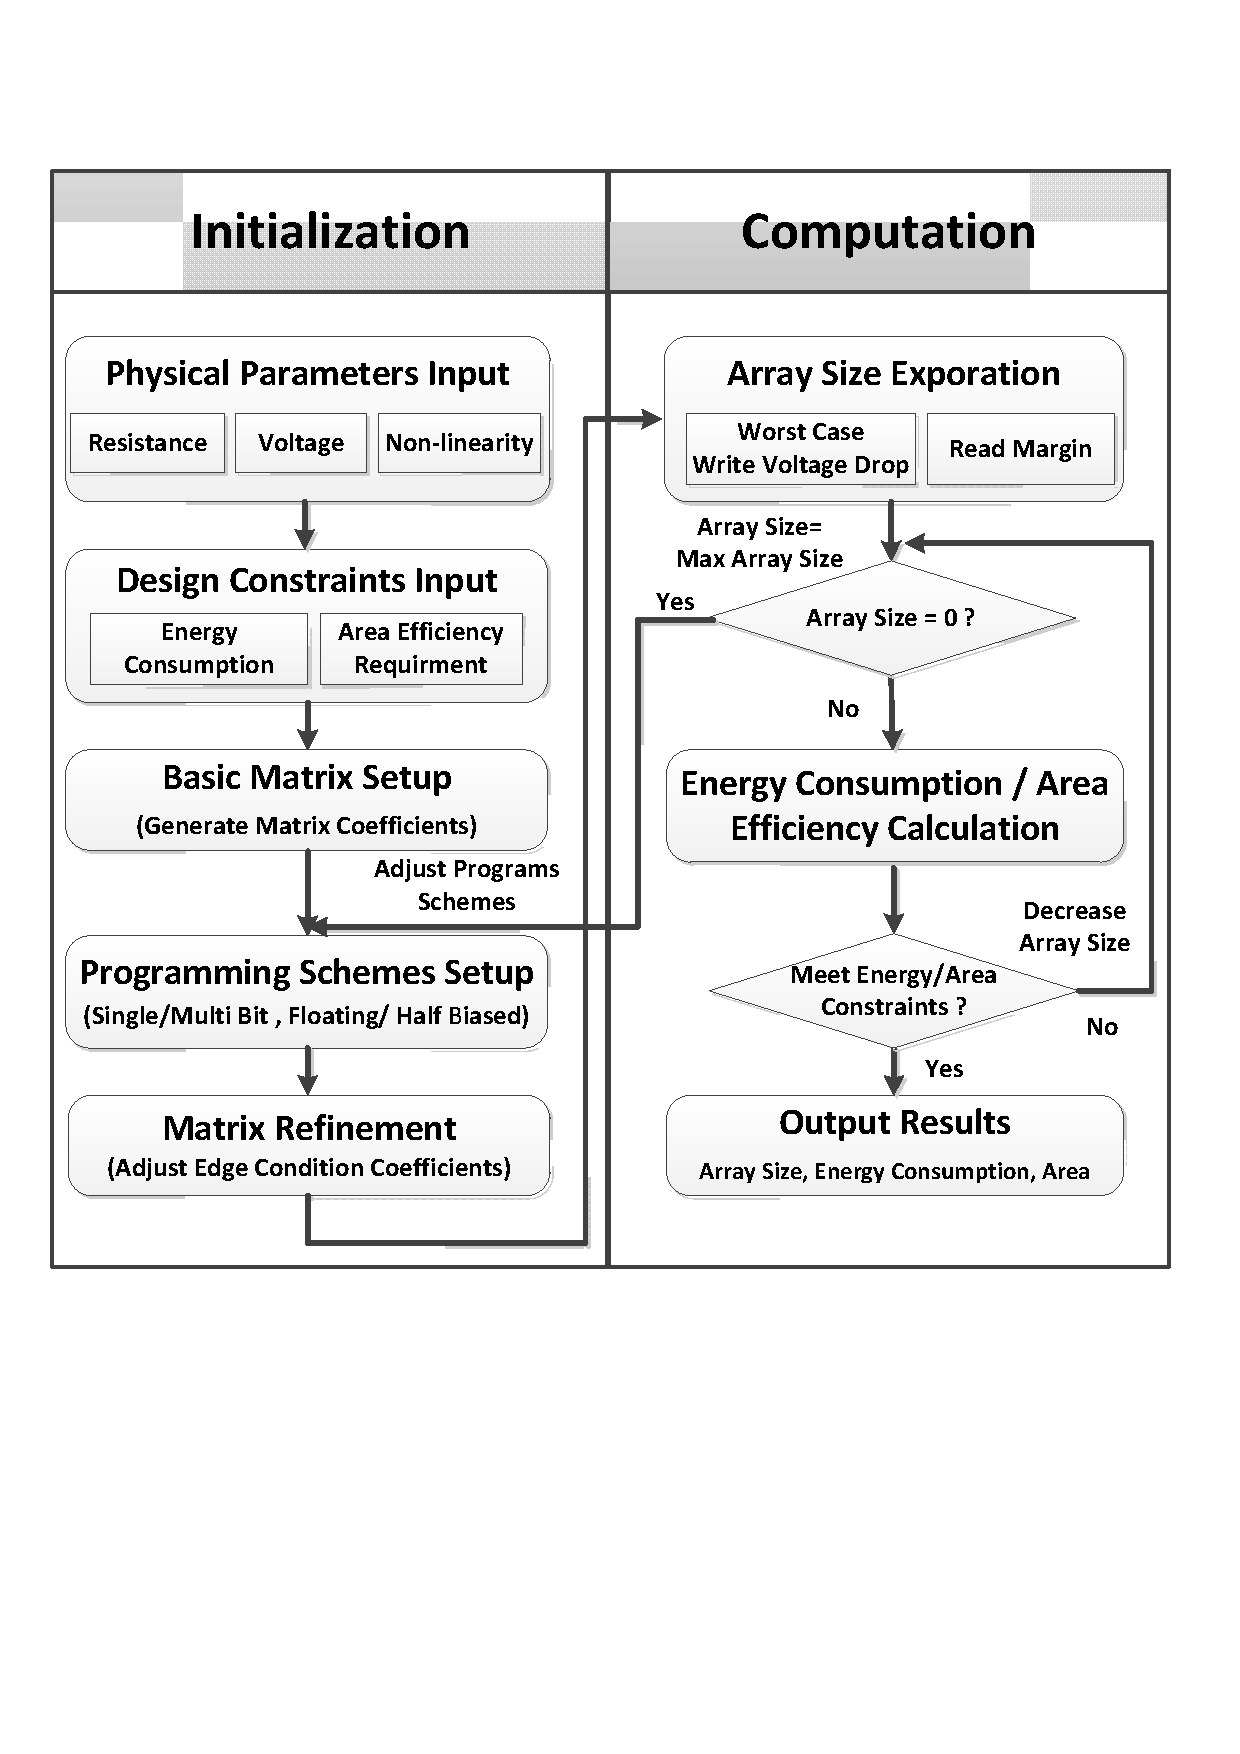
\includegraphics[width=0.5\textwidth]{./figures/FlowChart.pdf}\\
  \caption{The Proposed Design Flow of Design Space Exploration for ReRAM based Cross-point Array.}\label{fig:FlowChart}
  \vspace{-10pt}
\end{figure}
